% !TeX root=main.tex
% دستور زیر باعث شماره‌بندی صفحات فصول از ۱ می‌شود و باید در اولین فصل شما باشد. آن را حذف نکنید!
\pagenumbering{arabic} % 1, 2, ...

\chapter{مقدمه}
% دستور زیر باعث عدم‌نمایش شماره صفحه در اولین صفحه‌ی این فصل می‌شود.
%\thispagestyle{empty}
\ifDataveillance
  \textit{کریستین فوکس}
  \LTRfootnote{Christian Fuchs}
  جامعه شناس اتریشی،
  \textit{
    \gls{Social networking service}
  }
  \!({\lr{SNS}})
  در دنیای مدرن را به یک
  \textit{
    \gls{Panopticon}
  }
  تشبیه می کند   که در آن شرکت‌های بزرگی مانند
  \textit{
    \gls{Alphabet}
  }
  \!(
  شرکت مادر سرویس
  \textit{
    \gls{Google}
  }
  \!)
  و
  \textit{
    \gls{Meta}
  }
  \!(
  \!شرکت مادر و مالک برنامه‌های نرم‌افزاری مانند
  \textit{
    \gls{Instagram}
  }،
  \textit{
    \gls{Facebook}
  }
  و
  \textit{
    \gls{Whatsapp}
  }
  \!)
  به
  \textit{
    \gls{Dataveillance}
  }
  اعضا می‌پردازند
  \!\citep{romelePanopticismNotEnough2017a}.
  عبارت
  \textit{
    \gls{Panopticon}
  }
  را اولین بار
  \textit{
    \gls{Jeremy Bentham}
  }
  \!
  \citep{benthamPanopticonInspectionHouseContaining1791}
  برای توصیف ساختار‌های اجتماعی که مانند سیستم متمرکز نظارت عمل می‌کنند، از معماری وارد
  \textit{
    \gls{Social philosophy}
  }
  کرد
  \!(تصویر \ref{fig:MillbankPlan})
  \!\citep{holfordAccountGeneralPenitentiary1828}.
  \begin{figure}[ht]
    \centerline{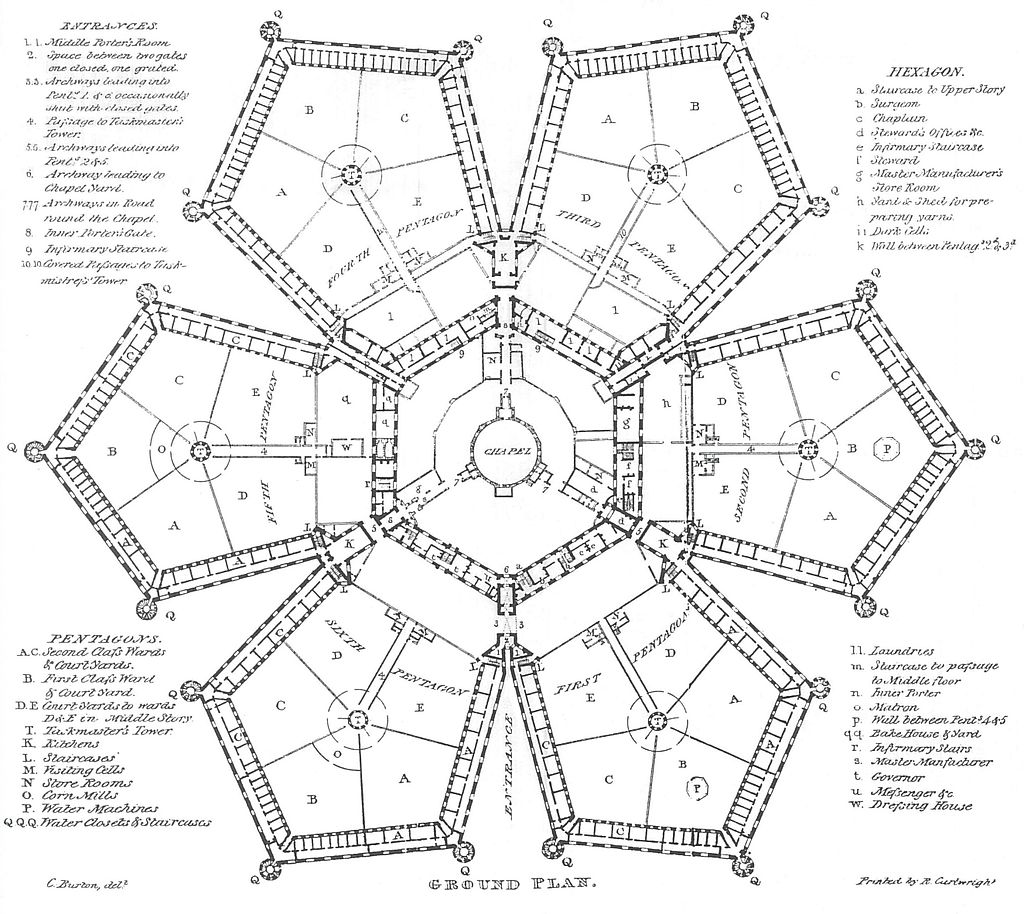
\includegraphics[width=0.8\textwidth]{MillbankPlan}}
    \caption{نقشه زندان \textit{
      \gls{Millbank}
    } مبتنی بر طراحی  \textit{
      \gls{Panopticon}
    }
      %\citep{kim2016integrated}
    }
    \label{fig:MillbankPlan}
  \end{figure}\\

\fi %Dataveillance
% * from old proposal and thesis fron khordad 1400 /media/d_drive/PJ/K/C/PJ-HDD-NiliLab/ssd2-laptop-backup-4mordad00/PJ/KN/Cog/proposal/tex/003
به نظر می‌رسد تصمیم‌گیرندگانی که در چنین سازمان‌هایی حضور دارند به حجم زیادی از اطلاعات
شخصی افراد دسترسی دارند. اگر این اطلاعات که در ابتدا با رضایت افراد و فقط جهت بهینه سازی ارائه خدمات مورد توافق جمع‌آوری شده‌است، با نهادهای ثانویه
به اشتراک گذاشته شود، می‌تواند برای نظارت و تغییر رفتار هدفمند استفاده شود. به این ترتیب
\textit{
  \gls{Social networking service}
}
به طور غیر مستقیم و بالقوه سبب ساز تغییرات اجتماعی خارج از کنترل و آگاهی کاربران شبکه های اجتماعی، که فراهم کنندگان و صاحبان اصلی
اطلاعات هستند، می‌شوند.
افراد تصمیم‌گیرنده در این سازمان‌ها به علت وظیفه‌ای که در قبال سازمان
متبوع خود دارند، ملزم به حداکثر کردن سود بنگاه‌های اقتصادی‌ای هستند
که مالکیت این سازمان‌ها و سرویس‌های ارائه شده را، در اختیار
دارند. تصمیم در به اشتراک گذاری اطلاعات از سوی این افراد، معمولا در وهله اول می‌تواند بر اساس چنین انگیزه‌ای مطابق با قواعد نظام‌های سرمایه‌داری و منطقی به نظر برسد.
اما از طرف دیگر، همین تصمیمات می‌تواند باعث متضرر شدن
کاربرانی باشد که مالک اصلی اطلاعات جمع‌آوری شده می‌باشند. در چنین شرایطی، وقتی که
\textit{
  \glspl{Oversight institution}
}
با تغییرات سریع  در ساختارهای
\textit{
  \glspl{Information society}
}
ناهماهنگ هستند
\!\citep{cavoukianDiscussionPaperPrivacy2009,machovaDiscourseSurveillancePrivacy2021}،
بررسی ساز و کار موثر بر تصمیمات این افراد، اهمیت پیدا می‌کند.


اهمیت  این موضوع زمانی بیشتر می‌شود که کاربران
\textit{
  \gls{Social networking service}
}
تحت تاثیر
\textit{
  \glspl{Motivitions of}
}
متضاد قرار می‌گیرند و رفتاری را نشان می‌دهند که با عنوان
\textit{
  \gls{Privacy paradox}
}
شناخته می‌شود
\!\citep{barthPrivacyParadoxInvestigating2017}.
این تناقض به عدم تناسب میان رفتار کاربران شبکه‌های اجتماعی با آگاهی بالای آنها از پیامدهای این رفتارها، اشاره دارد.
این تناقض زمانی مشاهده می‌شود که کاربران شبکه‌های اجتماعی با وجود اهمیتی که برای حفظ
\textit{
  \gls{Information privacy}
}
قائل هستند،  باز هم بی‌محابا نسبت به  منتشر کردن اطلاعات شخصی خود
در شبکه‌های اجتماعی اقدام می‌کنند.

این رفتار حتی پس از روبرو شدن با
پیامدهای سوءاستفاده از این اطلاعات نیز کاهش چشمگیری نداشته است
\!\citep{hermesWhoQuitsPrivacyInvasive2021,wirthLazinessExplanationPrivacy2022}.
به نظر می‌رسد که جلوگیری از پیامدهای  نامطلوب سوءاستفاده از اطلاعات خصوصی کاربران و نقض
\textit{
  \gls{Information privacy}
}
از طریق مداخلاتی که در سطح رفتار کاربران انجام شود، با توجه به گسترش و تنوع جمعیتی،
دشوار خواهد بود. با این وجود،
\textit{
  \gls{Information privacy}
}
که به توانایی افراد
برای کنترل اطلاعات مربوط به آنها اشاره دارد
\!\citep{smithInformationPrivacyMeasuring1996}
در سال‌های اخیر بیشتر مورد توجه کاربرانی قرار گرفته است
که داده‌های آنها توسط
\textit{
  \glspl{Social networking service}
}
جمع‌آوری، طبقه‌بندی و تحلیل می شود
\!{\citep{wallOrganizationalViolationsExternally2016}.
\textit{
  \gls{Information privacy}
}
با اشتراک‌گذاری اطلاعات شخصی توسط صاحب اطلاعات، در تضاد نیست.
\textit{
  \gls{Information privacy}
}
داشتن کنترل بر روی اطلاعات بعد از به  اشتراک‌گذاری، می‌باشد.\citep{acquistiEconomicsPrivacy2016}}.
به اشتراک گذاری اطلاعات شخصی از دید صاحبان اولیه اطلاعات،
به عنوان یک رفتار اجتماعی ناخوشایند و بالقوه ناهنجار، شناسایی شده است
\citep{norbergCopingInformationRequests2014}،
اما به نظر می‌رسد چنین دیدگاهی با تعریفی که برای
\textit{
  \gls{Information privacy}
}
ارائه شد، در تضاد قرار می‌گیرد. اگر کاربران بتوانند بعد از
\textit{
  \gls{Disclosure}
}
اطلاعات خود، بر روی نحوه استفاده از آن کنترل داشته باشند،
\textit{
  \gls{Personal Information Sharing Behavior}
}
به تنهایی
اثرات مخربی در پی نخواهد داشت.  به علاوه
جمع‌آوری و پردازش اطلاعات می‌تواند نتایج سازنده‌ای، در سطح اجتماعی و فردی داشته باشد
\citep{rockenbachProvidingPersonalInformation2020}.
امروزه افرادی که در
\textit{
  \glspl{Information society}
}
فاقد
\textit{
  \glspl{information record}
}
کافی در
\textit{
  \gls{Big data}
}
باشند، از جهات مختلف مورد
\textit{
  \gls{Discrimination}
}
قرار می‌گیرند
\!\citep{favarettoBigDataDiscrimination2019,lermanBigDataIts2013}.
با این دیدگاه، به اشتراک گذاری اطلاعات شخصی توسط صاحب اطلاعات، نه تنها
ناسازگارانه نیست، بلکه به یک رفتار
\textit{
  \gls{Prosocial}
}
تبدیل می‌شود.

اطلاعات کاربران پس از
\textit{
  \gls{Disclosure}
}
در اختیار تصمیم‌گیرندگانی قرار می‌گیرد که در
\textit{
  \glspl{Social networking service}
}
مسئول جمع‌آوری، ذخیره‌سازی و پردازش اطلاعات هستند. به نظر می‌آید که حفظ
\textit{
  \gls{Information privacy}
}
و جلوگیری از اثرات مخرب اجتماعی و فردی سوءاستفاده از
اطلاعات شخصی انباشته شده، از طریق شناسایی عوامل موثر
بر تصمیم‌گیری این افراد و به اجرا در آوردن
مداخلات موثر در این سطح،نتایج بهتری در پی داشته باشد.

کاربران
\textit{
  \glspl{Social networking service}
}
پس از ارائه اطلاعات شخصی خود، خدماتی را از آن دریافت می‌کنند. همان‌طور که اشاره شد، این
تبادل میان کاربر و
\textit{
  \glspl{Social networking service}
}
مورد توافق طرفین است. شرایط حاکم بر این تبادل در توافق‌نامه‌ای
که در زمان عضویت به افراد ارائه می‌شود، مشخص شده است. به عنوان مثال
فرد در قبال اطلاعات شخصی خود از امکانات
\textit{
  \glspl{Social networking service}
}
برای برقراری ارتباط با دوستان خود استفاده می کند. او همچنین
با شروط دیگری که  برای عضویت لازم بوده است، موافقت کرده است. او
قبول کرده است که
\textit{
  \gls{Social networking service}
}
اطلاعات شخصی‌اش را در جهت ارائه تبلیغات هدفمند به کاربران، ذخیره کند
و مورد بازبینی و پردازش قرار دهد. اثرات مخرب این تبادل از زمانی شروع می شود که دریافت کننده اطلاعات، از
آن برای اهدافی به غیر از توافق اولیه استفاده کند و یا امکان این کار را برای یک شخص ثالث فراهم کند
\!{\citep{padyabExploringImpactsSecondary2018}}.

\textit{
  \gls{Secondary use of information}
}،
استفاده از اطلاعات شخصی برای اهدافی فراتر
از توافق اولیه، بعد از
\textit{
  \gls{Disclosure}
}
اطلاعات شخصی توسط خود فرد، است. این عمل توسط موسسه جمع‌آوری کننده اطلاعات
و افراد تصمیم‌گیرنده در آن انجام می‌گیرد
\!{\citep{culnanHowDidThey1993}}.
پیامد‌های زیانبار تصمیمات بنگاه‌های اقتصادی و فن‌آوری بزرگی
مانند
\textit{
  \glspl{Meta}
}
برای استفاده ثانویه از اطلاعات شخصی جمع‌آوری شده، در پژوهش‌های مختلف بررسی شده اند
\!{\citep{padyabExploringImpactsSecondary2018}}.
این تصمیمات در سال‌های ۲۰۱۵ تا ۲۰۱۸، منجر به ناهنجاری‌های وسیع در سطح جوامع شدند.
پیامدهای این ناهنجاری‌ها در نهایت افراد عضو جوامع را به طور غیر مستقیم
تحت تاثیر قرار می‌دهند. این افراد، متشکل از همان کاربرانی هستند که به طور جمعی، تامین کننده
داده‌های جمع‌آوری شده توسط
\textit{
  \glspl{Meta}
}
بوده‌اند.
\!{\citep{redmanDataCredibilityProblem2013,dezwartSurveillanceBigData2014,spiekermannNetworksControlReport2016,schyffDuplicitousSocialMedia2020}}.
با وجود آسیب‌پذیری افراد از داده‌های شخصی جمع‌آوری شده توسط شرکت‌ها
و شرکای تجاری آنها، تحقیقات نشان می‌دهد
که کاربران این جنبه تبادل اطلاعات خود را نادیده می‌گیرند
\!{\citep{raynes-goldieAliasesCreepingWall2010,brandtzaegTooManyFacebook2010,youngPrivacyProtectionStrategies2013}}،
هرچند با توجه به تاثیرات سازنده‌ای که برای رفتار اشتراک گذاری اطلاعات در بخش‌های
قبلی نام برده شده است، به نظر می‌رسد که می‌توان، عدم تغییر رفتار کاربران در به اشتراک گذاری اطلاعات خود را
\textit{
  \gls{post–Cambridge Analytica scandal era}
}
\!{\citep{epsteinViewFramingDigital2021}}
، پدیده مطلوبی توصیف کرد. با این وجود وقوع چنین پدیده‌هایی به
\textit{
  \gls{Trust}
}
در افراد جامعه آسیب می‌زند و در نهایت سبب کاهش منافع جمعیِ جمع‌آوری و پردازش اطلاعات، می‌گردد.


\gls{Cambridge Analytica scandal}
در سال ۲۰۱۶ باعث پی‌گیری‌ حقوقی شرکت
\glspl{Meta}
و مدیرعامل آن
\textit{
  \gls{Mark Zuckerberg}
}
و محکومیت به پرداخت جریمه پنج میلیارد دلاری، شد
.\!{\citep{daviesFacebookPay5bn2019,smoutFacebookAgreesPay2019}}
واکنش مسؤولین فیسبوک نشان می‌دهد
که افراد تصمیم گیرنده در شرکت‌های جمع‌آوری کننده
اطلاعات نیز احتمالا از پیامدهایی که سیاست‌گذاری‌های آنها در استفاده ثانویه از اطلاعات شخصی کاربران
برای خود شرکت در پی دارد، ناآگاه هستند
\!{\citep{grewalSuspendingCambridgeAnalytica2018,kozlowskaFacebookDataPrivacy2018}}
\!. با توجه به اینکه این افراد مسؤول حداکثر
کردن سود شرکت‌های خود هستند،
به نظر می‌رسد که چنین تصمیماتی فرض
\glspl{Rational}
بودن عامل‌های تصمیم‌گیرنده در
\glspl{Rational choice theory}
را به چالش می‌کشد. با در نظر گرفتن این مساله‌، ما در این پژوهش از از یک چارچوب نظری که فرض
\textit{
  \gls{Rational}
}
بودن تصمیمات را به چالش می‌کشد برای
\textit{
  \glspl{Articulation}
}
مفاهیم و رویکردهایمان استفاده کردیم.

\section{نظریه رفتار برنامه‌ریزی‌شده و اهمیت استفاده ثانویه از اطلاعات}
تحقیقات زیادی برای بررسی رفتار کسانی که
اطلاعات خود را در اینترنت به اشتراک می‌گذارند انجام شده است
\!\!{\citep{kamleitnerInformationSharingPrivacy2019,kamleitnerYourDataMy2019}}.
همچنین رفتار افرادی که در مالکیت اطلاعت با فرد دیگر، شریک هستند بررسی شده است
\!\!{\citep{tawnieInterdependentPrivacy2017}}.
نتایج نشان می‌دهد که با وجود اینکه در همه جهان
\!،
\textit{
  \gls{Privacy}
}
اطلاعات شخصی افراد مساله مهمی برای کاربران آنلاین
است، بیشتر کاربران به ندرت برای محافظت از این داده، به خود زحمت می‌دهند و حتی در
بیشتر مواقع به طور داوطلبانه آن‌را پخش می‌کنند. تلاش زیادی انجام شده است تا این
دوگانگی میان
\textit{
  \gls{Privacy Attitude}
}
و رفتار، که معمولا با عنوان
\textit{
  \gls{Privacy paradox}
}
شناخته می‌شود، توضیح داده شود
\!{\citep{gerberExplainingPrivacyParadox2018}}.
به طور مشابه پژوهشی که در زمینه رفتار
\textit{
  \gls{Trust}
}
با به کار بردن
\textit{
  \gls{Theory of planned behavior}
}
در
\textit{
  \gls{Trust game}
}
انجام شده است،  وجود چنین تناقضی را در افراد
\textit{
  \gls{Trustor}
}
نیز نشان می‌دهد
\!\citep{gazdagNotWantTrust2019}.
به طور کلی، تا کنون  تحقیقات زیادی در حوزه
\textit{
  \gls{Information privacy}
}،
از
\textit{
  \gls{Trust game}
}
برای بررسی رفتار افراد در این تعامل
\textit{
  \gls{Interpersonal}
}،
استفاده کرده اند. با وجود اینکه تا به امروز رفتار کاربرانی که اطلاعات
\!(یا اطلاعات مشترک)
خود را به اشتراک می‌گذارند، مورد کنکاش قرار گرفته است، حیطه
رفتاری افرادی که دریافت کننده این  اطلاعات هستند به ندرت
مورد توجه قرار گرفته است
\!\citep{demmersYourDataAre2021}. 

با توجه به این موضوع و برای بررسی مسیر‌های بالقوه پژوهشی که می‌توانند به نتایج قابل استفاده منتهی شوند، رویکرد \textit{
  \gls{Exploratory}
} را انتخاب کردیم. 
در این روش تلاش کردیم تا ماهیت رفتار استفاده ثانویه از اطلاعات شخصی دیگران را در چارچوب نظریه‌ مطرح شده و بر
اساس فرضیه‌های پژوهشی، روشن کنیم. 

% \subsection{کمبریج آنالیتیکا و استفاده ثانویه از اطلاعات}
\subsection*{کمبریج آنالیتیکا و استفاده ثانویه از اطلاعات}
در سال ۲۰۱۳ استاد دانشگاه کمبریج یک برنامه به نام
«\lr{thisisyourdigitallife}»
ساخت. این برنامه در شبکه اجتماعی فیسبوک به کاربران
آزمون‌های شخصیت‌شناسی ارائه می‌کرد. وقتی کاربر فیسبوک برنامه را بر روی حساب کاربری خود فعال و نصب
می‌کرد، برنامه جمع‌آوری اطلاعات شخصی او را آغاز می‌کرد. این اطلاعات شامل اطلاعات حساب کاربری و فعالیت‌های کاربر در فیسبوک
بود. فعالیت‌هایی مانند اینکه کاربر کدام محتوای فیسبوک را لایک کرده است. در حدود سیصد هزار نفر این
برنامه را نصب کردند. اما اطلاعاتی که جمع‌آوری شد، به این تعداد محدود نماند.
این برنامه اطلاعاتی درباره دوستان کاربر که تنظیمات حریم خصوصی خود را درست  تنظیم نکرده بودند، را
نیز جمع‌آوری کرد. در نتیجه برنامه توانست به اطلاعات ۸۷ میلیون نفر دست یابد
\!\citep{kangFacebookSaysCambridge}.

سپس دکتر کوگان داده جمع‌آوری شده را به شرکت
\textit{
  \gls{ Strategic Communication Laboratories (SCL)}
}
که مالک شرکت کمبریج آنالیتیکا است، انتقال داد. این شرکت یک موسسه مشاوره
سیاسی بود که از داده برای شناسایی ویژگی‌های شخصیتی و رفتار رای دهندگان
استفاده می‌کرد
\!\citep{rosenbergHowTrumpConsultants2018}.
این شرکت از این داده برای کمک به پویش محافظه‌کاران برای هدف
قرار دادن تبلیغات اینترنتی و پیام رسان‌ها استفاده کرد. دکتر کوگان با این عمل، شرایط و مقررات فیسبوک را نقض کرد که انتقال یا
فروش داده را به هر شبکه تبلیغاتی ، دلال داده یا هر سرویس تبلیغاتی
و درآمد‌زایی، ممنوع می‌کرد
\!\citep{granvilleFacebookCambridgeAnalytica2018}.

وقتی در سال ۲۰۱۵ فیسبوک از این موضوع مطلع شد، برنامه دکتر کوگان
را حذف  کرد و از کوگان و کمبریج آنالیتیکا درخواست کرد که
مدرکی ارائه دهند، که داده را پاک کرده‌اند. کوگان و کمبریج آنالیتیکا
به فیسبوک تاییده‌ای ارائه دادند که داده را حذف کرده‌اند. هرچند  کپی داده
خارج از کنترل فیسبوک باقی ماند.  وقتی الکساندر نیکس، مدیر عامل
کمبریج آنالیتیکا، به قانون‌گذاران گفت که شرکتش داده‌های فیسبوک را در
اختیار ندارد، یکی از کارمندان او فاش کرد که اخیرا صدها گیگابایت داده رمزنگاری نشده را
بر روی سرورهای کمبریج آنالیتیکا دیده‌است.

در سال ۲۰۱۵، فیسبوک هیچ بیانیه عمومی‌ای درباره این رخداد منتشر نکرد و
کاربرانی که اطلاعات‌شان با کمبریج آنالیتیکا به اشتراک گذاشته شده
بود را مطلع نساخت. همچنین فیسبوک به کمیته تجارت فدرال، درباره این موضوع
چیزی نگفت. بر اساس آنچه که مارک زاکربرگ در کنفرانس دو روزه
استماع‌اش در نهم و دهم آوریل ۲۰۱۸ گفت، به محض اینکه گواهی کمبریج آنالیتیکا
مبنی بر حذف و تعهد عدم استفاده از داده را دریافت کردند، فیسبوک
موضوع را خاتمه یافته تلقی کرده‌است
\!\citep{spanFacebookCEOMark}.

با منتشر شدن این داستان در مارس ۲۰۱۸ در دو نشریه بین‌المللی، فیسبوک
مطلع شد که داده تا آن روز پاک نشده بوده است. نتایج به بار آمده
چنین حادثه‌ای بی سابقه بود. فیسبوک توسط چند نهاد قضایی در ایالت متحده،
جزیره انگلستان و اتحادیه اروپا مورد بازخواست قضایی قرار گرفت. یک پویش
فیسبوک را حذف کنید راه افتاد و افت شدید قیمت سهام باعث شد تقریبا پنجاه میلیارد دلار
سرمایه شرکت در عرض سه روز پس از فاش شدن اخبار، از بین برود.

% ^ %%%%%%%%%%%%%%%%%%%%%%%%%%%%%%%%%%%%%%%%%%%%%%%%%%%%%%%%%%%%%
% \section{اهمیت}
%% توضیح بیشتر اضافه گردد بعدا
پژوهش انجام شده در سال ۲۰۲۰ نشان می دهد که در بازار داده های خصوصی آنلاین بازیگران زیادی به عنوان واسطه وجود دارند.
\!\citep{agogoInvisibleMarketOnline2021}
همچنین با گسترش هر روزه سیستم های اطلاعاتی که به
جمع‌آوری، ذخیره‌سازی، پردازش و به‌اشتراک‌گذاری داده‌های
خصوصی افراد می‌پردازند، بررسی فرایندهای
تصمیم گیری و پارامتر‌های تاثیر گذار
بر این تصمیم‌گیری دارای اهمیت شده است
\!\citep{spiekermannValuesEthicsInformation2022}.
نظر به تاثیر ویژگی‌های شخصیتی افراد و توانایی های شناختی آنها بر روی تصمیم‌گیری اجتماعی که اعتمادپذیری اهمیت پیدا 
می‌کند، ویژگی‌های تاریک شخصیت شامل ماکیاولیسم، روانپریشی و خودشیفتگی را اندازه‌گیری کردیم.

از سوی دیگر نگرش افراد تصمیم گیرنده نسبت به ارزش اطلاعات خصوصی افراد می تواند نقش مهمی در رفتار آنها داشته باشد.
پژوهش‌هایی برای اندازه‌گیری ارزش داده‌های خصوصی انجام شده است
\!\citep{  fastValuePersonalData2021a,wesselsSellNotSell2019,tangHowChineseWeb2021}
\ifWillingnessToPay
  مقایسه میان رفتار افراد در پژوهش‌های اندازه‌گیری
  \textit{تمایل به پرداخت}
  \LTRfootnote{willingness to pay}
  نشان داده است که
  \textit{تمایل به پرداخت }
  با استفاده از روش‌های فرضی مانند
  \textit{ارزشيابی مشروط}
  \LTRfootnote{contingent valuation}
  که با استفاده از فرم‌های نظرسنجی انجام می‌شوند،
  میان ۱۷ تا ۶۳ درصد بالاتر
  از روشهای غیر فرضی مانند
  \textit{حراج تجربی}
  \LTRfootnote{experimental auction}
  است.
  حراج تجربی به عنوان یک روش
  \textit{سازگار با انگیزه}
  \LTRfootnote{incentive compatibility}
  شناسایی شده‌است
  \!\citep{martinez-carrascoComparingHypotheticalNonhypothetical2015}
  .
  یک فرایند،
  \textit{سازگار با انگیزه}
  است وقتی‌که همه شرکت‌کنندگان فقط  با درنظر گرفتن ترجیهات واقعی خود، بهترین خروجی را بدست می‌آورند
  \!\citep{nisanAlgorithmicGameTheory2007}
  \!. 
با توجه به انتخاب رویکرد اکتشافی در انجام این پژوهش و عدم  امکان پرداخت به شرکت‌کنندگان، از روش ارزشیابی مشروط 
مبتنی بر فرم نظرسنجی استفاده شد.
%  همچنین بررسی تاثیر شرایط درک شده اجتماعی-اقتصادی بر روی فرایند ارزشگذاری با استفاده از 
%  زیرمعیار‌های مرتبط با سطح رفاه بر اساس سیاهه کیفیت زندگی سازمان بهداشت جهانی انجام شد.

  % ^ %%%%%%%%%%%%%%%%%%%%%%%%%%%%%%%%%%%%%%%%%%%%%%%%%%%%%%%%%%%%%
  % ^ %%%%%%%%%%%%%%%%%%%%%%%%%%%%%%%%%%%%%%%%%%%%%%%%%%%%%%%%%%%%%
  % ^ %%%%%%%%%%%%%%%%%%%%%%%%%%%%%%%%%%%%%%%%%%%%%%%%%%%%%%%%%%%%%
\fi
\section{نظریه‌ها}
\textit{
  \gls{Rational choice theory}
}
\!{\citep{beckerEconomicApproachHuman1978}}،
این فرض را بنا می‌نهد که انسان‌ها بر اساس
تابعی از مجموع منفعت، با کسر مجموع هزینه‌های یک تصمیم
یا مبادله و برای حداکثر کردن فایده  شخصی دست به عمل می‌زنند.

این موضوع پایه‌ای برای طرح 
\textit{
  \gls{Theory of reasoned action}
}
توسط
\textit{
  \gls{Icek Ajzen}
}
و
\textit{
  \gls{Martin Fishbein}
}
در در دهه ۸۰ میلادی شد. این نظریات پیشنهاد می‌کنند که بین
\textit{
  \gls{Atteutude}
}
و رفتار رابطه وجود دارد
\!{\citep{ajzenPredictionGoaldirectedBehavior1986}}.
فهم رفتار اختیاری افراد به وسیله
بررسی انگیزه‌هایی که باعث اجرای یک عمل می شود، هدف اصلی این نظریه بود. این نظریه
بیان می کند که قصد اجرای یک عمل پیش‌بینی‌کننده اصلی انجام یا عدم ایجاد رفتار  است. به
علاوه پارامتر هنجاری
(هنجارهای اجتماعی که عمل را احاطه کرده‌اند)
در اجرا شدن یا نشدن عمل نقش بازی می کند
\!{\citep{doswellTestingTheoryReasoned2011,ajzenAttitudesAttitudeBehaviorRelation2000}}.
اما تحقیقاتی که در قالب چارچوب‌های
\textit{
  \gls{Behavioral economics}
}
انجام شد، این فرض را مورد تردید قرار داده اند
\!\citep{henrichEconomicManCrosscultural2005}.
برای رفع کاستی‌های
\textit{
  \gls{Theory of reasoned action}
}
آیزن در سال ۱۹۹۱
\!\citep{ajzenTheoryPlannedBehavior1991}
\textit{
  \gls{Theory of planned behavior}
}
را مطرح کرد. به بیان این تئوری سه پارامتر اصلی
\textit{
  \gls{Attitude}
}
\!،
\textit{\gls{Subjective norm}}
و
\textit{\gls{Perceived Behavioral control}}
\!،
\textit{\glspl{Behavioral intention}}
افراد را شکل می‌بخشند. پایه تفکر
\textit{
  \gls{Theory of planned behavior}
}
این است که
\textit{
  \gls{Personal Information Sharing Behavior}
}
از تعامل
\textit{\glspl{Psychological construct}}
\textit{
  \gls{Attitude}
}
\!،
\textit{\gls{Subjective norm}}،
\textit{\gls{Perceived Behavioral control}}
و
\textit{\glspl{Behavioral intention}}
نسبت به
\textit{
  \gls{Personal Information Sharing}
}،
ایجاد می‌شود.

در پژوهش‌های پیشین برای بررسی
\textit{
  \gls{Personal Information Sharing Behavior}
}
کاربران در زمان فاش‌سازی اطلاعات خود،از
\textit{
  \gls{Theory of reasoned action}
}
\!\citep{malhotraInternetUsersInformation2004}،
و
\textit{
  \gls{Theory of planned behavior}
}
برای ایجاد ساختاری که روابط بین پارامترها را مدل می‌کند، استفاده شده است
\!\citep{dinevExtendedPrivacyCalculus2006b}.

در این پژوهش ما بررسی رفتار به اشتراک گذاری اطلاعات خصوصی دیگران در
\textit{
  \gls{Conceptual framework}
}
\textit{
  \gls{Theory of planned behavior}
}
پرداختیم.

برای سنجش رویکرد‍ افراد به
\textit{
  \gls{Personal information of Others}
}
یک پرسشنامه بر اساس دسته‌بندی‌های هفت‌گانه‌ای که در پژوهش پیشین با توجه به رویکرد صاحبان
اولیه اطلاعات خصوصی نسبت به خطر فاش شدن اطلاعات شخصی شان در حوزه‌های مختلف، ساخته شد.
این پرسشنامه برای هر دسته از سوالات دارای ۲ سوال است. برای اینکه بتوان باور
آزمودنی‌ها، را هم بر اساس ارزش ذهنی خود
\!(نگرش به ارزش اطلاعات)
و هم بر اساس ارزش ذهنی دیگران
\!(هنجار ذهنی و باور هنجاری)
و همچنین برای اندازه‌گیری پایایی درونی،
سوالات به دو دسته تقسیم ‌می‌شود.
به هر آزمودنی، دسته اول اطلاعات خصوصی به همراه یک سوال برای سنجش باور هنجاری، و دسته دوم
اطلاعات به همراه سوال دیگر برای سنجش باور شخصی، ارائه شد. به طور تصادفی این دو دسته از
سوالات برای هر آزمودنی جابجا شدند تا در نهایت پاسخ‌های نیمی از آزمونی‌ها به دسته اول سوالات از دید خود و نیمی
دیگر از آزمودنی ها به دسته دوم سوالات از دید خود، جمع‌آوری شوند. به همین ترتیب پاسخ به سوالات دسته اول و دوم
با توجه به باور هنجاری از دو دسته مستقل به تصادف انتخاب شدند، جمع‌آوری شد. تصادفی سازی در زمان ورود آزمودنی‌ها
به آزمایش با انتصاب افراد با احتمال ۵۰ درصد به دو گروه، و توسط کتابخانه ری‌اکت جاوااسکریپت انجام شد.
% * %%%%%%%%%%%%%%%%%%%%%%%%%%%%%%%%%%%%%%%%%% from old proposal and thesis from khordad 1400

\section{متغیر‌ها و پرسشنامه‌ها}

\ifPlennedBahaviorTheory
  \textit{\gls{Theory of planned behavior}}
  \!(TPB)
  % \LTRfootnote{Theory of planned behavior (TPB) }
  %  acronyms اضافه شود
  ، تعامل سه باور فردی شامل
  \textit{\gls{Atteutude}} ،
  \textit{\gls{Subjective norm}} و
  \textit{\gls{Perceived Behavioral control}}
  % \LTRfootnote{Perceived Behavioral control}
  را عامل رفتار می داند
  \!(شکل: \ref{fig:Theory_of_planned_behavior_chart})
  \!\citep{ajzenTheoryPlannedBehavior2020}.
  در این نظریه
  \textit{\gls{Atteutude}}
  از دو نگرش احساسی و نگرش ابزاری تشکیل شده است.
  \textit{\gls{Subjective norm}}
  شامل  هنجارهای ذهنی و هنجار توصیفی است.
  \textit{\gls{Perceived Behavioral control}}،
  دو بخش کنترل رفتاری درک شده و خود کارآمدی درک شده را شامل می باشد
  در این نظریه عامل اصلی تعیین کننده
  رفتار، قصد رفتاری است و اجزای ساختاری این نظریه
  بر روی قصد تاثیر ویژه‌ای دارند
  \citep{mhmdpwrBrrsyTthyrTywry2022}
  \begin{figure}[ht]
    \centerline{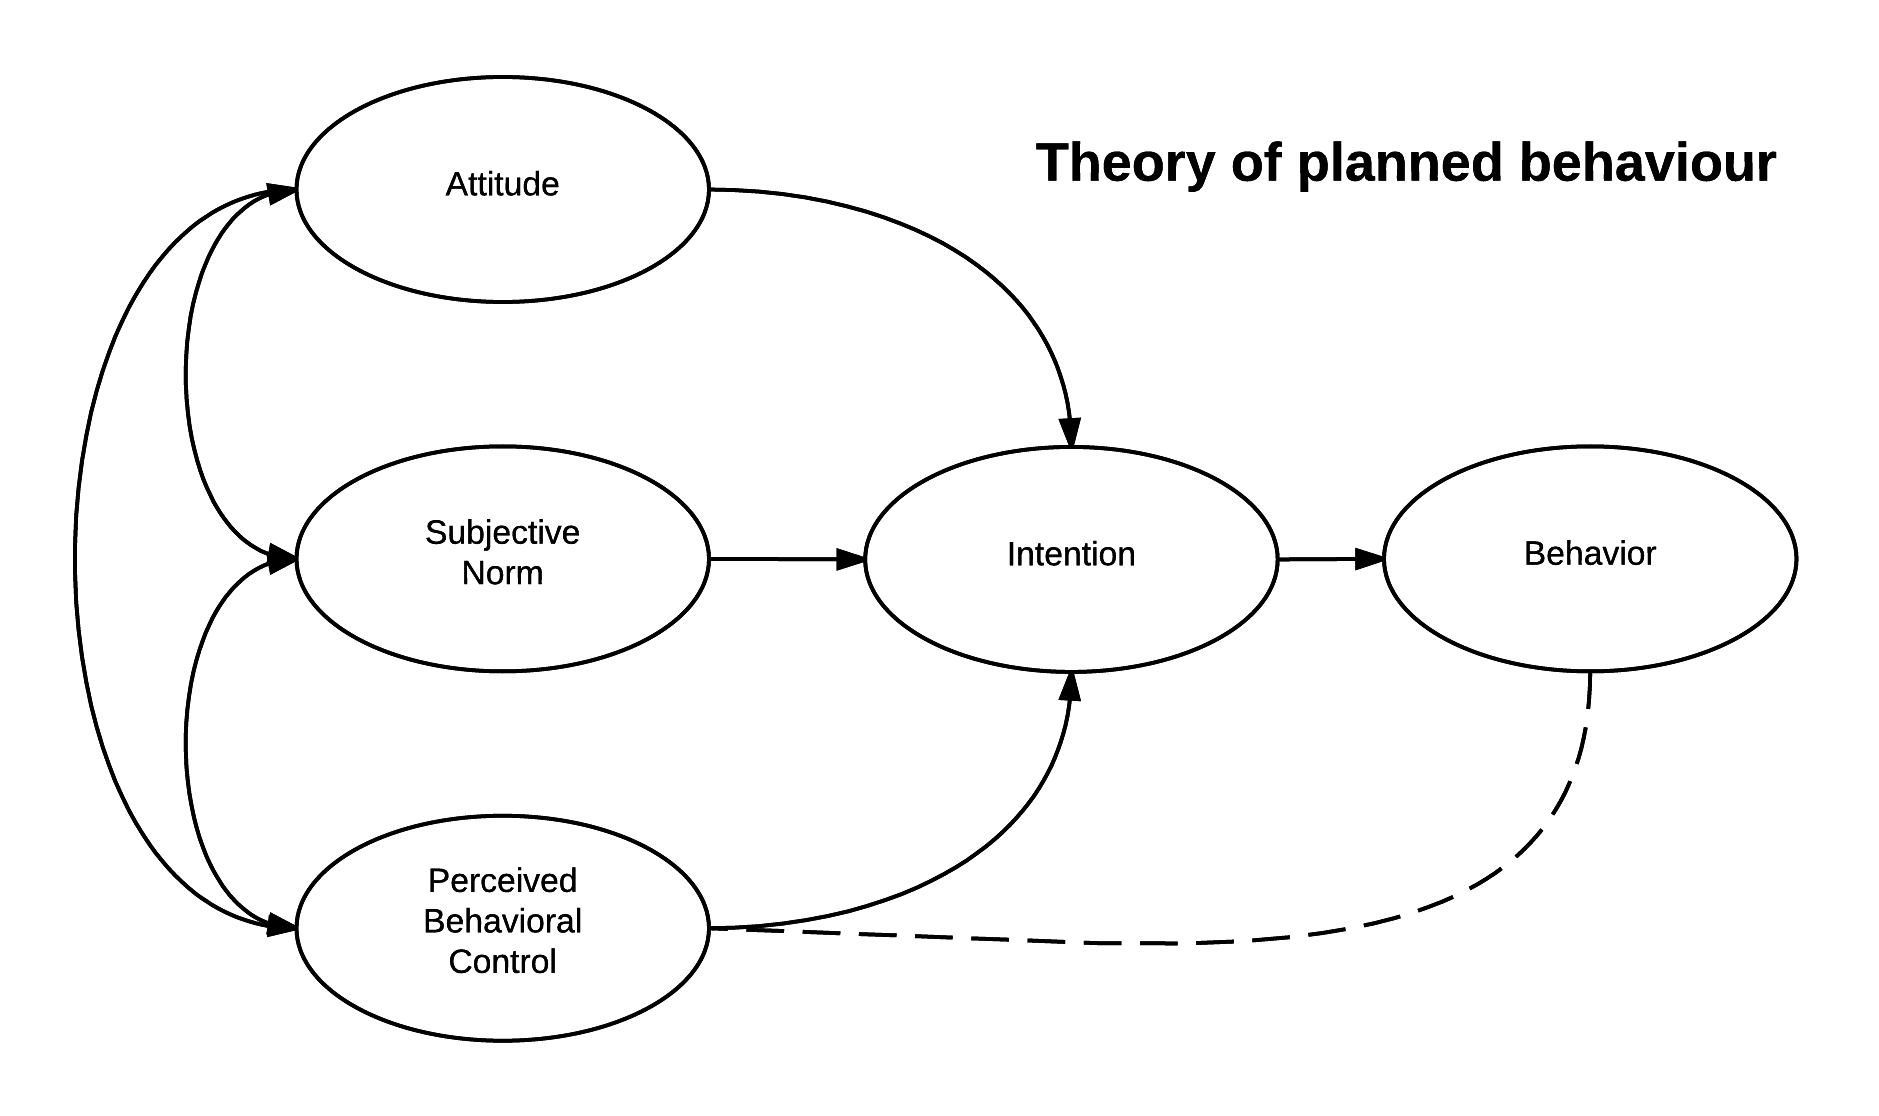
\includegraphics[width=0.8\textwidth]{Theory_of_planned_behavior_chart}}
    \caption{ساختار نظریه رفتار برنامه ریزی شده
      %\citep{kim2016integrated}
    }
    \label{fig:Theory_of_planned_behavior_chart}
  \end{figure}\\

  این نظریه در پژوهش‌های پیشین برای بررسی رفتار
  به اشتراک گذاری داده های خصوصی
  فرد در شبکه اجتماعی فیسبوک استفاده شده است
  \!\citep{vanderschyffInformationPrivacyBehavior2020}
  \!.
  مدل
  \gls{Theory of planned behavior}،
    احتمال وقوع  رفتار‌های ارادی، مخصوصا رفتار‌های ارادی مثبت را به شدت تمایل فرد به
  انجام آن رفتار مرتبط کرده‌است. به گفته
  \gls{Icek Ajzen}
  عامل تعیین کننده فرد برای انجام یک کار تمایلات او است.
\fi
%%%%%%%%%%%%%%%%%%%%

% \ifSurveyfillingBehavior
%   % بررسی اینکه آیا از نحوه پر کردن فرم ها می توان به کانفیدنس صداقت آزمودنی پی برد یا نه
%   در صورتیکه گزینه‌های پرسشنامه اجباری باشند کیفیت داده‌های جمع‌آوری شده کاهش می یابد.
%   \!\citep{sischkaImpactForcedAnswering2022}
% \fi

% ^ %%%%%%%%%%%%%%%%%%%%%%%%%%%%%%%%%%%%%%%%%%%%%%%%%%%%%%%%%%%%%
% ^ %%%%%%%%%%%%%%%%%%%%%%%%%%%%%%%%%%%%%%%%%%%%%%%%%%%%%%%%%%%%%
% ^ %%%%%%%%%%%%%%%%%%%%%%%%%%%%%%%%%%%%%%%%%%%%%%%%%%%%%%%%%%%%%

\section{فرضیه پژوهشی}
این آزمایش در دو بخش  طراحی شد. انجام بخش اول که فرضیه های اصلی به شکل شبه آزمایشی مورد سنجش قرار گرفتند، اجباری بود. بخش دوم بیشتر ماهیت 
\textit{
      \gls{Exploratory}
    }
داشت. این بخش به عنوان
\textit{
      \gls{Pilot study}
    }
  انتخاب و  بهینه سازی مدل رفتاری-شناختی مناسب برای تصمیم‌گیری در به اشترک گذاری بر اساس 
\textit{
      \gls{TPB}
    }

\subsection*{فرضیه‌های اصلی}
% ^ %%%%%%%%%%%%%%%%%%%%%%%%%%%%%%%%%%%%%%%%%%%%%%%%%%%%%%%%%%%%%
% ^ %%%%%%%%%%%%%%%%%%%%%%%%%%%%%%%%%%%%%%%%%%%%%%%%%%%%%%%%%%%%%
% ^ %%%%%%%%%%%%%%%%%%%%%%%%%%%%%%%%%%%%%%%%%%%%%%%%%%%%%%%%%%%%%

در ادامه این پایان‌نامه، در بخش دوم گزارشی از پژوهش‌های پیشین مرتبط با موضوع این پایان‌نامه ارائه می‌شود.
در بخش سوم روش انجام تحقیق انجام شده توضیح داده می شود
\!.
تعریف عملیاتی و نظری متغیر‌های اندازه‌گیری شده در این آزمایش، روش نمونه‌گیری و معرفی ابزارها و پرسشنامه‌ها در این بخش قرار دارند
\!.
سپس در بخش چهارم نتایج کمی به دست آمده پس از انجام آزمایش از اطلاعات جمع آوری شده، ارائه می‌شوند
\!.
در این بخش  روش به کار رفته برای تحلیل داده‌ها و آزمون فرضیه‌های پژوهشی و نتایج  به دست آمده، درج  می‌شوند
\!.
نمودار‌هایی تولید شده برای نمایش کیفی نتایج نیز در بخش چهارم هستند.
در بخش پنجم با در نظر گرفتن پژوهش‌های انجام شده و نظریه‌های موجود و شرایط و محدودیت‌های این پژوهش و ویژگی‌های نمونه، نتایج گزارش شده در بخش چهارم مورد بحث و بررسی
قرار می‌گیرند و پیشهادهایی برای پژوهش‌های آینده ارائه می‌شوند.

در بخش ابتدایی این پایان‌نامه تلاش کردیم تا روند شکل گیری سوال پژوهشی و اهمیت آن را توضیح دهیم.
همچنین نظریه‌هایی که برای توصیف رفتار افراد وجود دارند را معرفی کردیم و از آن‌ها به عنوان راهنمایی
برای ارائه فرضیه‌های پژوهشی مرتبط با سوال‌ مطرح شده، استفاده کردیم.
همچنین، پژوهش‌های انجام شده که مبنای نظریه‌های توصیف کننده رفتار به اشتراک گذاری اطلاعات خصوصی دیگران
بوده‌اند، به اختصار معرفی شدند. در بخش بعد، به مرور پژوهش‌هایی می‌پردازیم که با سوال پژوهشی و فرضیه‌های این پایان‌نامه مرتبط هستند.